\documentclass[11pt]{article}
\usepackage{amsmath, amssymb, mathtools, bm}
\usepackage{physics}
\usepackage{tikz}
\usetikzlibrary{arrows.meta, calc, positioning, decorations.pathmorphing}
\usepackage{pgfplots}
\pgfplotsset{compat=1.18}
\usepackage[margin=2.3cm]{geometry}
\usepackage{siunitx}
\usepackage{booktabs}
\usepackage{hyperref}
\usepackage{braket}

\newcommand{\de}{\mathrm{d}}
\newcommand{\kB}{k_{\mathrm{B}}}
\newcommand{\TF}{T_{\mathrm{F}}}
\newcommand{\TD}{\theta_{\mathrm{D}}}
\newcommand{\EF}{E_{\mathrm{F}}}
\newcommand{\kF}{k_{\mathrm{F}}}
\newcommand{\kD}{k_{\mathrm{D}}}
\newcommand{\omD}{\omega_{\mathrm{D}}}

\title{B6: Condensed-Matter Physics --- 2015 Model Solutions}
\author{Trinity Term 2015 (Paper A13485W1)}
\date{}

\begin{document}
\maketitle

%==========================================================
\section*{Question 1 --- Fermi/Debye temperatures and electronic vs. lattice heat capacity}

\textbf{Problem.} Monovalent metal: $n$ atoms (and electrons) per unit volume; sound speed $c$. Derive $\TF$ and $\TD$, sketch $C_e$, derive $C_{\mathrm{ph}}$ for $T\ll\TD$, and apply to Cu (fcc, $a=\SI{0.36}{nm}$, $c=\SI{2700}{m\,s^{-1}}$, $A=\pi^2/2$).

\subsection*{(a) Fermi and Debye temperatures}

Free-electron sphere: each $\mathbf k$-state occupies $(2\pi)^3/V$ in $\mathbf k$-space; spin degeneracy $2$:
\[
n = \frac{2}{(2\pi)^{3}}\,\frac{4\pi \kF^{3}}{3}.
\]
Solve for $\kF$:
\[
\kF = (3\pi^{2} n)^{1/3}.
\]
Fermi energy:
\[
\EF = \frac{\hbar^{2}\kF^{2}}{2 m_{e}} = \frac{\hbar^{2}}{2 m_{e}}(3\pi^{2} n)^{2/3}.
\]
Definition $\kB \TF = \EF$:
\[
\boxed{\;\TF = \frac{\hbar^{2}}{2 m_{e}\kB}(3\pi^{2} n)^{2/3}.\;}
\]

Debye sphere fills the Brillouin zone with $3N$ phonon modes; $3$ polarisations, density $V/(2\pi)^{3}$:
\[
3 n = \frac{3}{(2\pi)^{3}}\,\frac{4\pi \kD^{3}}{3}.
\]
Solve for $\kD$:
\[
\kD = (6\pi^{2} n)^{1/3}.
\]
Linear dispersion $\omD = c\,\kD$:
\[
\omD = c\,(6\pi^{2} n)^{1/3}.
\]
Definition $\kB \TD = \hbar\omD$:
\[
\boxed{\;\TD = \frac{\hbar c}{\kB}(6\pi^{2} n)^{1/3}.\;}
\]

\subsection*{(b) Electronic heat capacity --- simple argument}

At $T\ll\TF$, only electrons within $\sim\kB T$ of $\EF$ are thermally active. Number of such electrons per unit volume:
\[
\Delta n \sim n\,\frac{\kB T}{\EF} = n\,\frac{T}{\TF}.
\]
Each gains thermal energy $\sim\kB T$:
\[
u \sim \Delta n\cdot \kB T \sim n\,\kB T\,\frac{T}{\TF}.
\]
Differentiate w.r.t.\ $T$:
\[
\boxed{\;C_{e} = \pdv{u}{T} = A\,n\,\kB\!\left(\frac{T}{\TF}\right),\;}
\]
with $A$ an $O(1)$ constant ($A=\pi^{2}/2$ from the exact Sommerfeld expansion).

\subsection*{(c) Debye assumptions and low-$T$ phonon heat capacity}

Assumptions:
\begin{itemize}\setlength\itemsep{0pt}
\item Linear, isotropic dispersion $\omega = c\,k$ (one effective sound speed).
\item Single Debye cutoff $\kD$ chosen so that the total number of modes equals $3N$.
\item Phonons are quantised harmonic oscillators (Bose statistics).
\end{itemize}

Mode density (3 polarisations):
\[
g(\omega)\,\de\omega = \frac{3}{(2\pi)^{3}}\cdot 4\pi k^{2}\,\de k,\qquad \omega = c\,k.
\]
Eliminate $k$:
\[
g(\omega) = \frac{3\omega^{2}}{2\pi^{2} c^{3}},\qquad 0\le\omega\le\omD.
\]
Internal energy per unit volume:
\[
u(T) = \int_{0}^{\omD}\!\hbar\omega\,n_{B}(\omega)\,g(\omega)\,\de\omega,\qquad n_{B}=\frac{1}{e^{\hbar\omega/\kB T}-1}.
\]
Substitute $g(\omega)$:
\[
u(T) = \frac{3\hbar}{2\pi^{2} c^{3}}\int_{0}^{\omD}\!\frac{\omega^{3}}{e^{\hbar\omega/\kB T}-1}\,\de\omega.
\]
Change variable $x=\hbar\omega/\kB T$:
\[
u(T) = \frac{3\hbar}{2\pi^{2} c^{3}}\!\left(\frac{\kB T}{\hbar}\right)^{4}\!\int_{0}^{\hbar\omD/\kB T}\!\frac{x^{3}}{e^{x}-1}\,\de x.
\]
Low-$T$ limit $T\ll\TD$: extend upper limit to $\infty$, use $\int_{0}^{\infty}\!x^{3}/(e^{x}-1)\,\de x = \pi^{4}/15$:
\[
u(T) = \frac{3\hbar}{2\pi^{2} c^{3}}\,\frac{(\kB T)^{4}}{\hbar^{4}}\,\frac{\pi^{4}}{15}.
\]
Use $\hbar\omD = \kB\TD$ and $\omD = c\kD$, so $c^{3} = (\kB\TD/\hbar)^{3}/\kD^{3}$ and $\kD^{3}=6\pi^{2} n$:
\[
\frac{1}{c^{3}} = \frac{\hbar^{3}\,6\pi^{2} n}{(\kB\TD)^{3}}.
\]
Substitute:
\[
u(T) = \frac{3\hbar}{2\pi^{2}}\cdot\frac{\hbar^{3}\,6\pi^{2} n}{(\kB\TD)^{3}}\cdot\frac{(\kB T)^{4}}{\hbar^{4}}\cdot\frac{\pi^{4}}{15}.
\]
Simplify:
\[
u(T) = \frac{3\pi^{4}}{5}\,n\,\kB T\,\!\left(\frac{T}{\TD}\right)^{3}.
\]
Differentiate:
\[
\boxed{\;C_{\mathrm{ph}} = \pdv{u}{T} = \frac{12\pi^{4}}{5}\,n\,\kB\!\left(\frac{T}{\TD}\right)^{3}\qquad (T\ll\TD).\;}
\]

\subsection*{(d) Numerical estimates for Cu}

Fcc, monovalent: $4$ atoms (and electrons) per conventional cell of side $a$:
\[
n = \frac{4}{a^{3}} = \frac{4}{(0.36\times 10^{-9})^{3}}\,\si{m^{-3}}.
\]
Numerator and denominator:
\[
a^{3} = 4.666\times 10^{-29}\,\si{m^{3}}.
\]
Divide:
\[
n = 8.57\times 10^{28}\,\si{m^{-3}}.
\]

Fermi temperature: $\TF = \hbar^{2}(3\pi^{2} n)^{2/3}/(2 m_{e}\kB)$.
\[
3\pi^{2} n = 3\times 9.870\times 8.57\times 10^{28} = 2.538\times 10^{30}\,\si{m^{-3}}.
\]
\[
(3\pi^{2} n)^{2/3} = (2.538\times 10^{30})^{2/3} = 1.861\times 10^{20}\,\si{m^{-2}}.
\]
\[
\hbar^{2}/(2 m_{e}\kB) = \frac{(1.055\times 10^{-34})^{2}}{2\times 9.11\times 10^{-31}\times 1.381\times 10^{-23}} = 4.42\times 10^{-16}\,\si{m^{2}\,K}.
\]
\[
\TF = 4.42\times 10^{-16}\times 1.861\times 10^{20}\,\si{K} = \SI{8.2e4}{K}.
\]

Debye temperature: $\TD = \hbar c\,(6\pi^{2} n)^{1/3}/\kB$.
\[
6\pi^{2} n = 5.076\times 10^{30}\,\si{m^{-3}}.
\]
\[
(6\pi^{2} n)^{1/3} = 1.719\times 10^{10}\,\si{m^{-1}}.
\]
\[
\hbar c/\kB = \frac{1.055\times 10^{-34}\times 2700}{1.381\times 10^{-23}} = 2.063\times 10^{-8}\,\si{m\,K}.
\]
\[
\TD = 2.063\times 10^{-8}\times 1.719\times 10^{10}\,\si{K} = \SI{354}{K}.
\]

\paragraph{Crossover $C_{e}=C_{\mathrm{ph}}$.} Equate the two with $A=\pi^{2}/2$:
\[
\frac{\pi^{2}}{2}\,n\kB\,\frac{T}{\TF} = \frac{12\pi^{4}}{5}\,n\kB\,\!\left(\frac{T}{\TD}\right)^{3}.
\]
Cancel $n\kB$:
\[
\frac{\pi^{2}}{2}\,\frac{T}{\TF} = \frac{12\pi^{4}}{5}\,\frac{T^{3}}{\TD^{3}}.
\]
Solve for $T^{2}$:
\[
T^{2} = \frac{5}{24\pi^{2}}\,\frac{\TD^{3}}{\TF}.
\]
Substitute numbers:
\[
T^{2} = \frac{5}{24\times 9.870}\times\frac{(354)^{3}}{8.23\times 10^{4}}\,\si{K^{2}}.
\]
Numerator $\TD^{3}=4.44\times 10^{7}\,\si{K^{3}}$, divide by $\TF$:
\[
\TD^{3}/\TF = 5.39\times 10^{2}\,\si{K^{2}}.
\]
Multiply by $5/(24\pi^{2}) = 0.02110$:
\[
T^{2} = 11.4\,\si{K^{2}}.
\]
Square root:
\[
\boxed{\;T_{\times} \approx \SI{3.4}{K}.\;}
\]
$C_{e}$ dominates for $T\lesssim T_{\times}\approx\SI{3.4}{K}$.

\paragraph{Ratio at \SI{300}{K}.}
\[
\frac{C_{e}}{C_{\mathrm{ph}}} = \frac{\pi^{2}/2}{12\pi^{4}/5}\,\frac{T/\TF}{(T/\TD)^{3}} = \frac{5}{24\pi^{2}}\,\frac{\TD^{3}}{\TF\,T^{2}}.
\]
Substitute $T=\SI{300}{K}$:
\[
\frac{C_{e}}{C_{\mathrm{ph}}} = 0.02110\times\frac{4.44\times 10^{7}}{8.23\times 10^{4}\times (300)^{2}}.
\]
Numerator $0.02110\times 4.44\times 10^{7}=9.37\times 10^{5}$; denominator $8.23\times 10^{4}\times 9\times 10^{4} = 7.41\times 10^{9}$:
\[
\boxed{\;\frac{C_{e}}{C_{\mathrm{ph}}}\bigg|_{\SI{300}{K}}\approx 1.3\times 10^{-4}.\;}
\]

%==========================================================
\section*{Question 2 --- Structure factor and powder XRD of Al, KCl, Si}

\textbf{Problem.} Define structure factor; relate to Bragg intensity. For Al, KCl, Si (all fcc) identify the strong rings with $h^{2}+k^{2}+l^{2}\le 16$ and discuss whether neutrons would change the count.

\subsection*{(a) Structure factor}

The structure factor is the Fourier amplitude of the unit-cell scattering density evaluated at a reciprocal lattice vector $\mathbf G_{hkl}$. For a unit cell with $N$ atoms at fractional coordinates $(x_{j},y_{j},z_{j})$ and atomic form factors $f_{j}$:
\[
\boxed{\;S_{(hkl)} = \sum_{j=1}^{N} f_{j}\,e^{2\pi i(h x_{j}+k y_{j}+l z_{j})}.\;}
\]
The Bragg peak intensity satisfies
\[
I_{(hkl)} \propto |S_{(hkl)}|^{2},
\]
multiplied by Lorentz, polarisation, and multiplicity factors. A reflection is absent (systematic absence) when $S_{(hkl)}=0$, which is how non-primitive lattices and specific bases are identified. X-rays scatter off electrons ($f_{j}\propto Z_{j}$ at low $|\mathbf q|$); neutrons scatter off nuclei (and unpaired spins) with $b_{j}$ varying irregularly with isotope. Different $f_{j}$ vs.\ $b_{j}$ patterns can change which weak reflections are visible.

\subsection*{(b) Allowed fcc reflections with $h^{2}+k^{2}+l^{2}\le 16$}

Lattice contribution: fcc lattice with basis at $(0,0,0)$, $(\tfrac12,\tfrac12,0)$, $(\tfrac12,0,\tfrac12)$, $(0,\tfrac12,\tfrac12)$ gives
\[
S_{\text{fcc}} = f\!\left[1 + e^{i\pi(h+k)} + e^{i\pi(h+l)} + e^{i\pi(k+l)}\right].
\]
Selection rule:
\[
S_{\text{fcc}} \neq 0\;\iff\;h,k,l\;\text{all even or all odd}.
\]
Enumerate $(hkl)$ with $h^{2}+k^{2}+l^{2}\le 16$ satisfying the rule:
\[
\begin{array}{c|c|c}
(hkl) & h^{2}+k^{2}+l^{2} & \\\hline
(111) & 3 & \\
(200) & 4 & \\
(220) & 8 & \\
(311) & 11 & \\
(222) & 12 & \\
(400) & 16 & \\
\end{array}
\]
Six rings.

\paragraph{Al (single atom, $f_{\mathrm{Al}}$).} All six reflections survive:
\[
\boxed{\;\text{Al rings: }(111),(200),(220),(311),(222),(400).\;}
\]

\paragraph{KCl: K at $(0,0,0)$, Cl at $(\tfrac12,0,0)$.} Combining basis with fcc:
\[
S_{(hkl)} = \!\left[f_{\mathrm K} + f_{\mathrm{Cl}}\,e^{i\pi h}\right]\!\left[1 + e^{i\pi(h+k)} + e^{i\pi(h+l)} + e^{i\pi(k+l)}\right].
\]
The basis bracket gives
\[
f_{\mathrm K}+f_{\mathrm{Cl}}(-1)^{h} = \begin{cases} f_{\mathrm K}+f_{\mathrm{Cl}}, & h\text{ even} \\ f_{\mathrm K}-f_{\mathrm{Cl}}, & h\text{ odd}.\end{cases}
\]
With Z(K)=19, Z(Cl)=17 the K and Cl ions are both isoelectronic with Ar ($Z=18$): $f_{\mathrm K^{+}}\approx f_{\mathrm{Cl}^{-}}$ to a good approximation. Hence for $h$ odd, $S\approx 0$. The (111) and (311) rings (which have all-odd indices) are extinguished:
\[
\boxed{\;\text{KCl strong rings: }(200),(220),(222),(400).\;}
\]

\paragraph{Si: basis at $(0,0,0)$ and $(\tfrac14,\tfrac14,\tfrac14)$ (diamond).} Basis bracket:
\[
1 + e^{i\pi(h+k+l)/2}.
\]
Modulus squared:
\[
|1+e^{i\pi(h+k+l)/2}|^{2} = \begin{cases} 4, & h+k+l\equiv 0\pmod 4 \\ 2, & h+k+l\;\text{odd} \\ 0, & h+k+l\equiv 2\pmod 4.\end{cases}
\]
Apply to the six fcc-allowed reflections:
\[
\begin{array}{c|c|c}
(hkl) & h+k+l & \text{basis factor}\\\hline
(111) & 3 & 2\quad\text{(weak/medium)}\\
(200) & 2 & 0\quad\text{extinct}\\
(220) & 4 & 4\quad\text{strong}\\
(311) & 5 & 2\quad\text{(weak/medium)}\\
(222) & 6 & 0\quad\text{extinct}\\
(400) & 4 & 4\quad\text{strong}\\
\end{array}
\]
The four observed (``strong'') rings are those with non-zero basis factor:
\[
\boxed{\;\text{Si rings: }(111),(220),(311),(400).\;}
\]

\subsection*{(c) Same with neutrons?}

\textbf{Al:} single atom basis, no extinctions from the basis $\Rightarrow$ same six rings.

\textbf{KCl:} the X-ray near-extinction of $h$-odd rings relied on $f_{\mathrm K^{+}}\approx f_{\mathrm{Cl}^{-}}$ (both Ar-like, $Z=18$). Neutron coherent scattering lengths are nuclear: $b_{\mathrm K}\approx\SI{3.7}{fm}$, $b_{\mathrm{Cl}}\approx\SI{9.6}{fm}$, so $b_{\mathrm K}\neq b_{\mathrm{Cl}}$:
\[
S_{(hkl)}^{h\text{ odd}} \propto b_{\mathrm K}-b_{\mathrm{Cl}}\;\neq 0.
\]
Hence the (111) and (311) rings reappear $\Rightarrow$ \emph{six} rings with neutrons.

\textbf{Si:} the diamond extinction $h+k+l\equiv 2\pmod 4$ is geometric (basis at $\frac14,\frac14,\frac14$) and independent of scattering length. With one element, the basis factor is the same up to a constant:
\[
\boxed{\;\text{Al: 6 (unchanged); KCl: 4}\to\text{6; Si: 4 (unchanged).}\;}
\]

%==========================================================
\section*{Question 3 --- Phonon dispersion with long-range springs}

\textbf{Problem.} Define phonon and a measurement method. For a 1D monatomic chain (period $a$, mass $M$) with Hooke's-law couplings $C_{n}$ to all neighbours, derive the equation of motion and dispersion. Then sketch and compare two specific chains.

\subsection*{(a) Definition and measurement}

A \emph{phonon} is the quantum of vibrational excitation of a crystal lattice: a normal-mode oscillation with wavevector $\mathbf k$ and angular frequency $\omega_{s}(\mathbf k)$ ($s$ a polarisation/branch label), carrying energy $\hbar\omega_{s}(\mathbf k)$ and crystal momentum $\hbar\mathbf k$ (defined modulo a reciprocal lattice vector).

\paragraph{Inelastic neutron scattering.} Conservation of energy and momentum:
\[
\mathbf k_{i}-\mathbf k_{f} = \mathbf G + \mathbf q,\qquad E_{i}-E_{f} = \pm\hbar\omega(\mathbf q).
\]
Measure $\mathbf k_{i}$, $\mathbf k_{f}$ and the energy transfer (e.g.\ triple-axis spectrometer) at fixed $\mathbf G$, scan $\mathbf q$, deduce $\omega(\mathbf q)$ along chosen high-symmetry directions.

\subsection*{(b) Equation of motion and dispersion}

Force on atom $p$ from atom $p+n$:
\[
F_{p,n} = C_{n}(u_{p+n}-u_{p}).
\]
Sum over all neighbours (force constant depends on $|n|$, $C_{-n}=C_{n}$):
\[
M\,\ddot u_{p} = \sum_{n\neq 0} C_{n}(u_{p+n}-u_{p}).
\]
Use $C_{-n}=C_{n}$ and split:
\[
M\,\ddot u_{p} = \sum_{n>0} C_{n}\!\left(u_{p+n}+u_{p-n}-2u_{p}\right).
\]
Plane-wave ansatz $u_{p} = U\,e^{i(kpa-\omega t)}$:
\[
-M\omega^{2} = \sum_{n>0} C_{n}\!\left(e^{ikna}+e^{-ikna}-2\right).
\]
Combine exponentials:
\[
-M\omega^{2} = \sum_{n>0} 2C_{n}\!\left[\cos(kna)-1\right].
\]
Apply $1-\cos(x) = 2\sin^{2}(x/2)$:
\[
M\omega^{2} = \sum_{n>0} 4C_{n}\sin^{2}\!\left(\frac{nka}{2}\right).
\]
Solve for $\omega$:
\[
\boxed{\;\omega(k) = \!\left(\frac{4}{M}\right)^{\!1/2}\!\left[\sum_{n>0}C_{n}\sin^{2}\!\left(\frac{nka}{2}\right)\right]^{1/2}.\;}
\]

\subsection*{(c) Two chains: nearest neighbour vs.\ NN+NNN}

\paragraph{Chain 1 (NN only, $C_{1}$).}
\[
\omega_{1}(k) = 2\sqrt{C_{1}/M}\,\bigl|\sin(ka/2)\bigr|.
\]

\paragraph{Chain 2 ($C_{1}$, $C_{2}=C_{1}/2$).}
\[
\omega_{2}(k) = \!\left(\frac{4 C_{1}}{M}\right)^{\!1/2}\!\left[\sin^{2}\!\left(\frac{ka}{2}\right)+\tfrac12\sin^{2}(ka)\right]^{1/2}.
\]

\paragraph{Sound speed.} Small-$k$ expansion: $\sin(nka/2)\approx nka/2$:
\[
\omega^{2} \approx \frac{4}{M}\sum_{n>0}C_{n}\!\left(\frac{nka}{2}\right)^{2} = \frac{(ka)^{2}}{M}\sum_{n>0}n^{2}C_{n}.
\]
Sound speed $v_{s}=\partial\omega/\partial k$ at $k\to 0$:
\[
v_{s} = a\!\left(\frac{1}{M}\sum_{n>0}n^{2}C_{n}\right)^{\!1/2}.
\]
Chain~1: $\sum n^{2}C_{n}=C_{1}$:
\[
v_{s,1} = a\sqrt{C_{1}/M}.
\]
Chain~2: $\sum n^{2}C_{n}=C_{1}+4\cdot(C_{1}/2)=3C_{1}$:
\[
v_{s,2} = a\sqrt{3C_{1}/M}.
\]
Ratio:
\[
\boxed{\;\frac{v_{s,2}}{v_{s,1}} = \sqrt{3}\approx 1.73.\;}
\]

\paragraph{Maximum frequency.} Chain~1: maximum at $ka=\pi$:
\[
\omega_{1,\max} = 2\sqrt{C_{1}/M}.
\]
Chain~2: $\omega_{2}^{2}(k)=(4C_{1}/M)\!\left[\sin^{2}(ka/2)+\tfrac12\sin^{2}(ka)\right]$. Use $\sin(ka)=2\sin(ka/2)\cos(ka/2)$:
\[
\omega_{2}^{2}(k) = \frac{4C_{1}}{M}\sin^{2}(ka/2)\!\left[1+2\cos^{2}(ka/2)\right].
\]
Let $s=\sin^{2}(ka/2)\in[0,1]$, then $\cos^{2}(ka/2)=1-s$:
\[
\omega_{2}^{2} = \frac{4C_{1}}{M}\,s\,(3-2s).
\]
Differentiate w.r.t.\ $s$:
\[
\dv{\omega_{2}^{2}}{s} = \frac{4C_{1}}{M}(3-4s).
\]
Stationary at $s=3/4$:
\[
\omega_{2,\max}^{2} = \frac{4C_{1}}{M}\cdot\frac{3}{4}\cdot\!\left(3-\tfrac{3}{2}\right) = \frac{4C_{1}}{M}\cdot\frac{9}{8} = \frac{9C_{1}}{2M}.
\]
Take square root:
\[
\omega_{2,\max} = \frac{3}{\sqrt{2}}\sqrt{C_{1}/M}.
\]
Ratio:
\[
\boxed{\;\frac{\omega_{2,\max}}{\omega_{1,\max}} = \frac{3/\sqrt{2}}{2} = \frac{3}{2\sqrt{2}}\approx 1.06.\;}
\]
The maximum lies inside the BZ at $\sin^{2}(ka/2)=3/4$, i.e.\ $ka=2\arcsin(\sqrt{3}/2)=2\pi/3$.

\paragraph{Sketch.}
\begin{center}
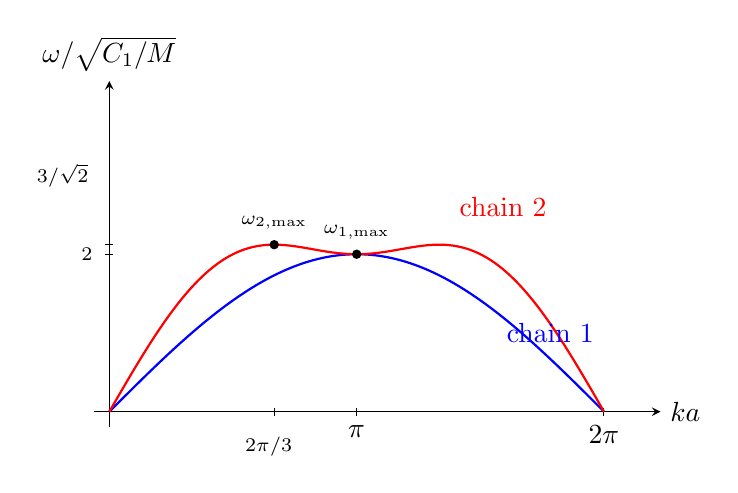
\begin{tikzpicture}[>=stealth, scale=1.0]
\draw[->] (-0.2,0) -- (7.0,0) node[right] {$ka$};
\draw[->] (0,-0.2) -- (0,4.2) node[above] {$\omega/\sqrt{C_{1}/M}$};
% ticks
\draw (3.14,0.05) -- (3.14,-0.05) node[below] {$\pi$};
\draw (6.28,0.05) -- (6.28,-0.05) node[below] {$2\pi$};
\draw (2.094,0.05) -- (2.094,-0.05) node[below=4pt,xshift=-2pt] {\scriptsize $2\pi/3$};
\draw (-0.05,2.0) -- (0.05,2.0) node[left=4pt] {\scriptsize $2$};
\draw (-0.05,2.121) -- (0.05,2.121);
\node[left=4pt] at (0,3.0) {\scriptsize $3/\sqrt{2}$};
% chain 1: 2 |sin(x/2)|
\draw[thick, blue, domain=0:6.28, samples=200, smooth] plot (\x, {2*abs(sin(\x*180/3.1416/2))});
% chain 2: 2 sqrt(s(3-2s)) with s=sin^2(x/2)
\draw[thick, red, domain=0:6.28, samples=200, smooth] plot (\x, {2*sqrt( (sin(\x*180/3.1416/2))^2 * (3 - 2*(sin(\x*180/3.1416/2))^2) )});
% markers at extrema
\node[circle,fill,inner sep=1.2pt,label=above:{\scriptsize $\omega_{1,\max}$}] at (3.1416,2.0) {};
\node[circle,fill,inner sep=1.2pt,label=above:{\scriptsize $\omega_{2,\max}$}] at (2.094,2.121) {};
% labels at end
\node[blue] at (5.6,1.0) {chain 1};
\node[red]  at (5.0,2.6) {chain 2};
\end{tikzpicture}
\end{center}

%==========================================================
\section*{Question 4 --- Intrinsic and doped Si: carriers, Hall coefficient}

\textbf{Problem.} Define intrinsic/extrinsic, derive $n(T)$ for an intrinsic semiconductor, define $R_{H}$ for one carrier type, and use Hall data on Si to extract $E_{g}$, then estimate p-type doping that pins $R_{H}$ over $\SI{300}{K}$--$\SI{500}{K}$.

\subsection*{(a) Intrinsic vs.\ extrinsic}

\textbf{Intrinsic.} Carrier concentrations determined solely by thermal excitation across the gap of the pure crystal: $n=p=n_{i}(T)$, $E_{F}$ near mid-gap.

\textbf{Extrinsic.} Carriers supplied by impurity (donor/acceptor) levels: at low/intermediate $T$ the dominant carrier type and concentration are set by the dopants, $n\neq p$, $E_{F}$ pinned near the dopant level.

\subsection*{(b) Conduction-band electron density}

Parabolic band $E(\mathbf k) = E_{c}+\hbar^{2}k^{2}/(2 m_{e}^{*})$. Density of states per unit volume:
\[
g_{c}(E) = \frac{1}{2\pi^{2}}\!\left(\frac{2 m_{e}^{*}}{\hbar^{2}}\right)^{\!3/2}\!(E-E_{c})^{1/2},\qquad E\ge E_{c}.
\]
Fermi--Dirac, non-degenerate ($E_{c}-E_{F}\gg\kB T$), Boltzmann tail:
\[
f(E) \approx e^{-(E-E_{F})/\kB T}.
\]
Electron density:
\[
n = \int_{E_{c}}^{\infty}\!g_{c}(E)\,f(E)\,\de E.
\]
Substitute $\epsilon = E-E_{c}$:
\[
n = \frac{1}{2\pi^{2}}\!\left(\frac{2 m_{e}^{*}}{\hbar^{2}}\right)^{\!3/2}\!e^{-(E_{c}-E_{F})/\kB T}\!\int_{0}^{\infty}\!\epsilon^{1/2}\,e^{-\epsilon/\kB T}\,\de\epsilon.
\]
Standard integral $\int_{0}^{\infty}\!\epsilon^{1/2}e^{-\epsilon/\kB T}\de\epsilon = (\sqrt{\pi}/2)(\kB T)^{3/2}$:
\[
n = 2\!\left(\frac{m_{e}^{*}\kB T}{2\pi\hbar^{2}}\right)^{\!3/2}\!e^{-(E_{c}-E_{F})/\kB T}.
\]
Define $N_{c}(T) = 2(m_{e}^{*}\kB T/2\pi\hbar^{2})^{3/2}$:
\[
n = N_{c}(T)\,e^{-(E_{c}-E_{F})/\kB T}.
\]
Analogous derivation for holes:
\[
p = N_{v}(T)\,e^{-(E_{F}-E_{v})/\kB T}.
\]
Intrinsic ($n=p\equiv n_{i}$): solve for $E_{F}$ to eliminate it:
\[
n_{i}^{2} = n p = N_{c}N_{v}\,e^{-E_{g}/\kB T},\qquad E_{g}=E_{c}-E_{v}.
\]
Take square root, absorb prefactors into a single constant $A$:
\[
\boxed{\;n_{i} = A\,T^{3/2}\,\exp\!\left(\frac{-E_{g}}{2\kB T}\right).\;}
\]

\subsection*{(c) Hall coefficient and $E_{g}$ from data}

Steady drift in crossed $\mathbf E$ (along $\hat x$), $\mathbf B$ (along $\hat z$): transverse field cancels Lorentz force on the majority carrier. For a single carrier type with charge $q$ (sign included) and density $n_{q}$:
\[
qE_{y} + q v_{x} B_{z} = 0,\qquad j_{x} = n_{q}\,q\,v_{x}.
\]
Eliminate $v_{x}$:
\[
E_{y} = -\frac{j_{x} B_{z}}{n_{q} q}.
\]
Definition $R_{H} = E_{y}/(j_{x} B_{z})$:
\[
\boxed{\;R_{H} = \frac{1}{n_{q}\,q}\;\left(=-\frac{1}{n e}\;\text{electrons},\; +\frac{1}{p e}\;\text{holes}\right).\;}
\]

\paragraph{Why electrons dominate $R_{H}$ in intrinsic Si.} With both carriers present, the two-carrier Hall coefficient is
\[
R_{H} = \frac{p\mu_{h}^{2}-n\mu_{e}^{2}}{e(p\mu_{h}+n\mu_{e})^{2}}.
\]
For intrinsic Si $n=p$ and $\mu_{e}\approx\SI{1350}{cm^{2}\,V^{-1}\,s^{-1}}$, $\mu_{h}\approx\SI{480}{cm^{2}\,V^{-1}\,s^{-1}}$, so $\mu_{e}^{2}\gg\mu_{h}^{2}$:
\[
R_{H}\approx -\frac{1}{n e}\,\frac{\mu_{e}^{2}-\mu_{h}^{2}}{(\mu_{e}+\mu_{h})^{2}} \approx -\frac{1}{n e}\,(1-\text{small}).
\]
Hence $|R_{H}|\approx 1/(n_{i} e)$ to within $\sim 20\%$ and is well-approximated by the electron-only formula.

\paragraph{Extracting $E_{g}$.} $|R_{H}|\propto 1/n_{i}\propto T^{-3/2}\exp(E_{g}/2\kB T)$:
\[
\frac{|R_{H}(300)|}{|R_{H}(500)|} = \!\left(\frac{500}{300}\right)^{\!3/2}\!\exp\!\left[\frac{E_{g}}{2\kB}\!\left(\frac{1}{300}-\frac{1}{500}\right)\right] = 4\times 10^{4}.
\]
Compute the prefactor:
\[
(500/300)^{3/2} = 2.152.
\]
Take log:
\[
\frac{E_{g}}{2\kB}\!\left(\frac{1}{300}-\frac{1}{500}\right) = \ln\!\left(\frac{4\times 10^{4}}{2.152}\right) = \ln(1.86\times 10^{4}) = 9.83.
\]
Compute the temperature factor:
\[
\frac{1}{300}-\frac{1}{500} = \frac{500-300}{300\times 500} = 1.333\times 10^{-3}\,\si{K^{-1}}.
\]
Solve for $E_{g}$:
\[
E_{g} = 2\kB\,\frac{9.83}{1.333\times 10^{-3}}.
\]
Numerical evaluation: $9.83/1.333\times 10^{-3}=7.37\times 10^{3}\,\si{K}$:
\[
E_{g} = 2\times 1.381\times 10^{-23}\times 7.37\times 10^{3}\,\si{J} = 2.04\times 10^{-19}\,\si{J}.
\]
Convert to eV ($1\,\mathrm{eV}=1.602\times 10^{-19}\,\si{J}$):
\[
\boxed{\;E_{g}\approx \SI{1.27}{eV}.\;}
\]
(The accepted value for Si is \SI{1.12}{eV}; the data quoted in the problem yield \SI{1.27}{eV}.)

\subsection*{(d) Doping for a sign-flipped, $T$-independent $R_{H}$}

Intrinsic $R_{H}$ is negative (electron-like). To flip the sign and pin $R_{H}$ over the whole range, dope with \emph{acceptors} (p-type) and require $p\approx N_{A}\gg n_{i}(T)$ throughout $\SI{300}{K}\le T\le\SI{500}{K}$. The intrinsic carrier density is largest at $\SI{500}{K}$:
\[
n_{i}(\SI{500}{K}) = \frac{1}{|R_{H}(\SI{500}{K})|\,e} = \frac{1}{(625/4\times 10^{4})\times 1.602\times 10^{-19}}.
\]
Numerator $|R_{H}(\SI{500}{K})| = \SI{1.5625e-2}{m^{3}\,C^{-1}}$. Multiply by $e$:
\[
|R_{H}|\,e = 1.5625\times 10^{-2}\times 1.602\times 10^{-19} = 2.503\times 10^{-21}\,\si{m^{3}}.
\]
Reciprocal:
\[
n_{i}(\SI{500}{K}) = 4.0\times 10^{20}\,\si{m^{-3}}.
\]
Minimum acceptor density (a comfortable factor of $\gtrsim 10$ above $n_{i}(500\,\mathrm{K})$ keeps $R_{H}$ flat):
\[
\boxed{\;N_{A}\gtrsim n_{i}(\SI{500}{K})\approx \SI{4e20}{m^{-3}}\;\text{(acceptors, p-type).}\;}
\]
Take $N_{A}\sim\SI{4e20}{m^{-3}}$ as the marginal estimate.

\paragraph{Electron concentration at \SI{300}{K}.} Mass-action $np = n_{i}^{2}$ with $p\approx N_{A}$, $n_{i}(\SI{300}{K})$ from the intrinsic Hall data:
\[
n_{i}(\SI{300}{K}) = \frac{1}{|R_{H}(\SI{300}{K})|\,e} = \frac{1}{625\times 1.602\times 10^{-19}}\,\si{m^{-3}}.
\]
Numerator product $625\times 1.602\times 10^{-19} = 1.001\times 10^{-16}$:
\[
n_{i}(\SI{300}{K}) = 9.99\times 10^{15}\,\si{m^{-3}}.
\]
Apply mass-action:
\[
n(\SI{300}{K}) = \frac{n_{i}^{2}(\SI{300}{K})}{N_{A}} = \frac{(9.99\times 10^{15})^{2}}{4.0\times 10^{20}}\,\si{m^{-3}}.
\]
Numerator $9.98\times 10^{31}$; divide:
\[
\boxed{\;n(\SI{300}{K}) \approx \SI{2.5e11}{m^{-3}}.\;}
\]

\end{document}
